\chapter{零零阁}

在荷塘南面,西湖北面,有一座小山。西边的山头上,有一座高大的阁子,唤作零零阁。%据说是以前“零零字班”的校友捐建的,因此得名。
1970年,适逢清华园学制由6年改为5年,两个年级的学生在同一年毕业。
当时校内习惯以毕业年份来作为届号,故早一年入学的称为“零字班”,晚一年入学的便称为“零零字班”。
这座阁子,便是由零零字班的校友捐建的。
阁子有两层,有着高高的螺旋台阶,矗立在山顶上,是这一范围内最高的建筑物,可以一览原来的皇家园林的秀美景观。

\begin{figure}[!b]
	\centering
	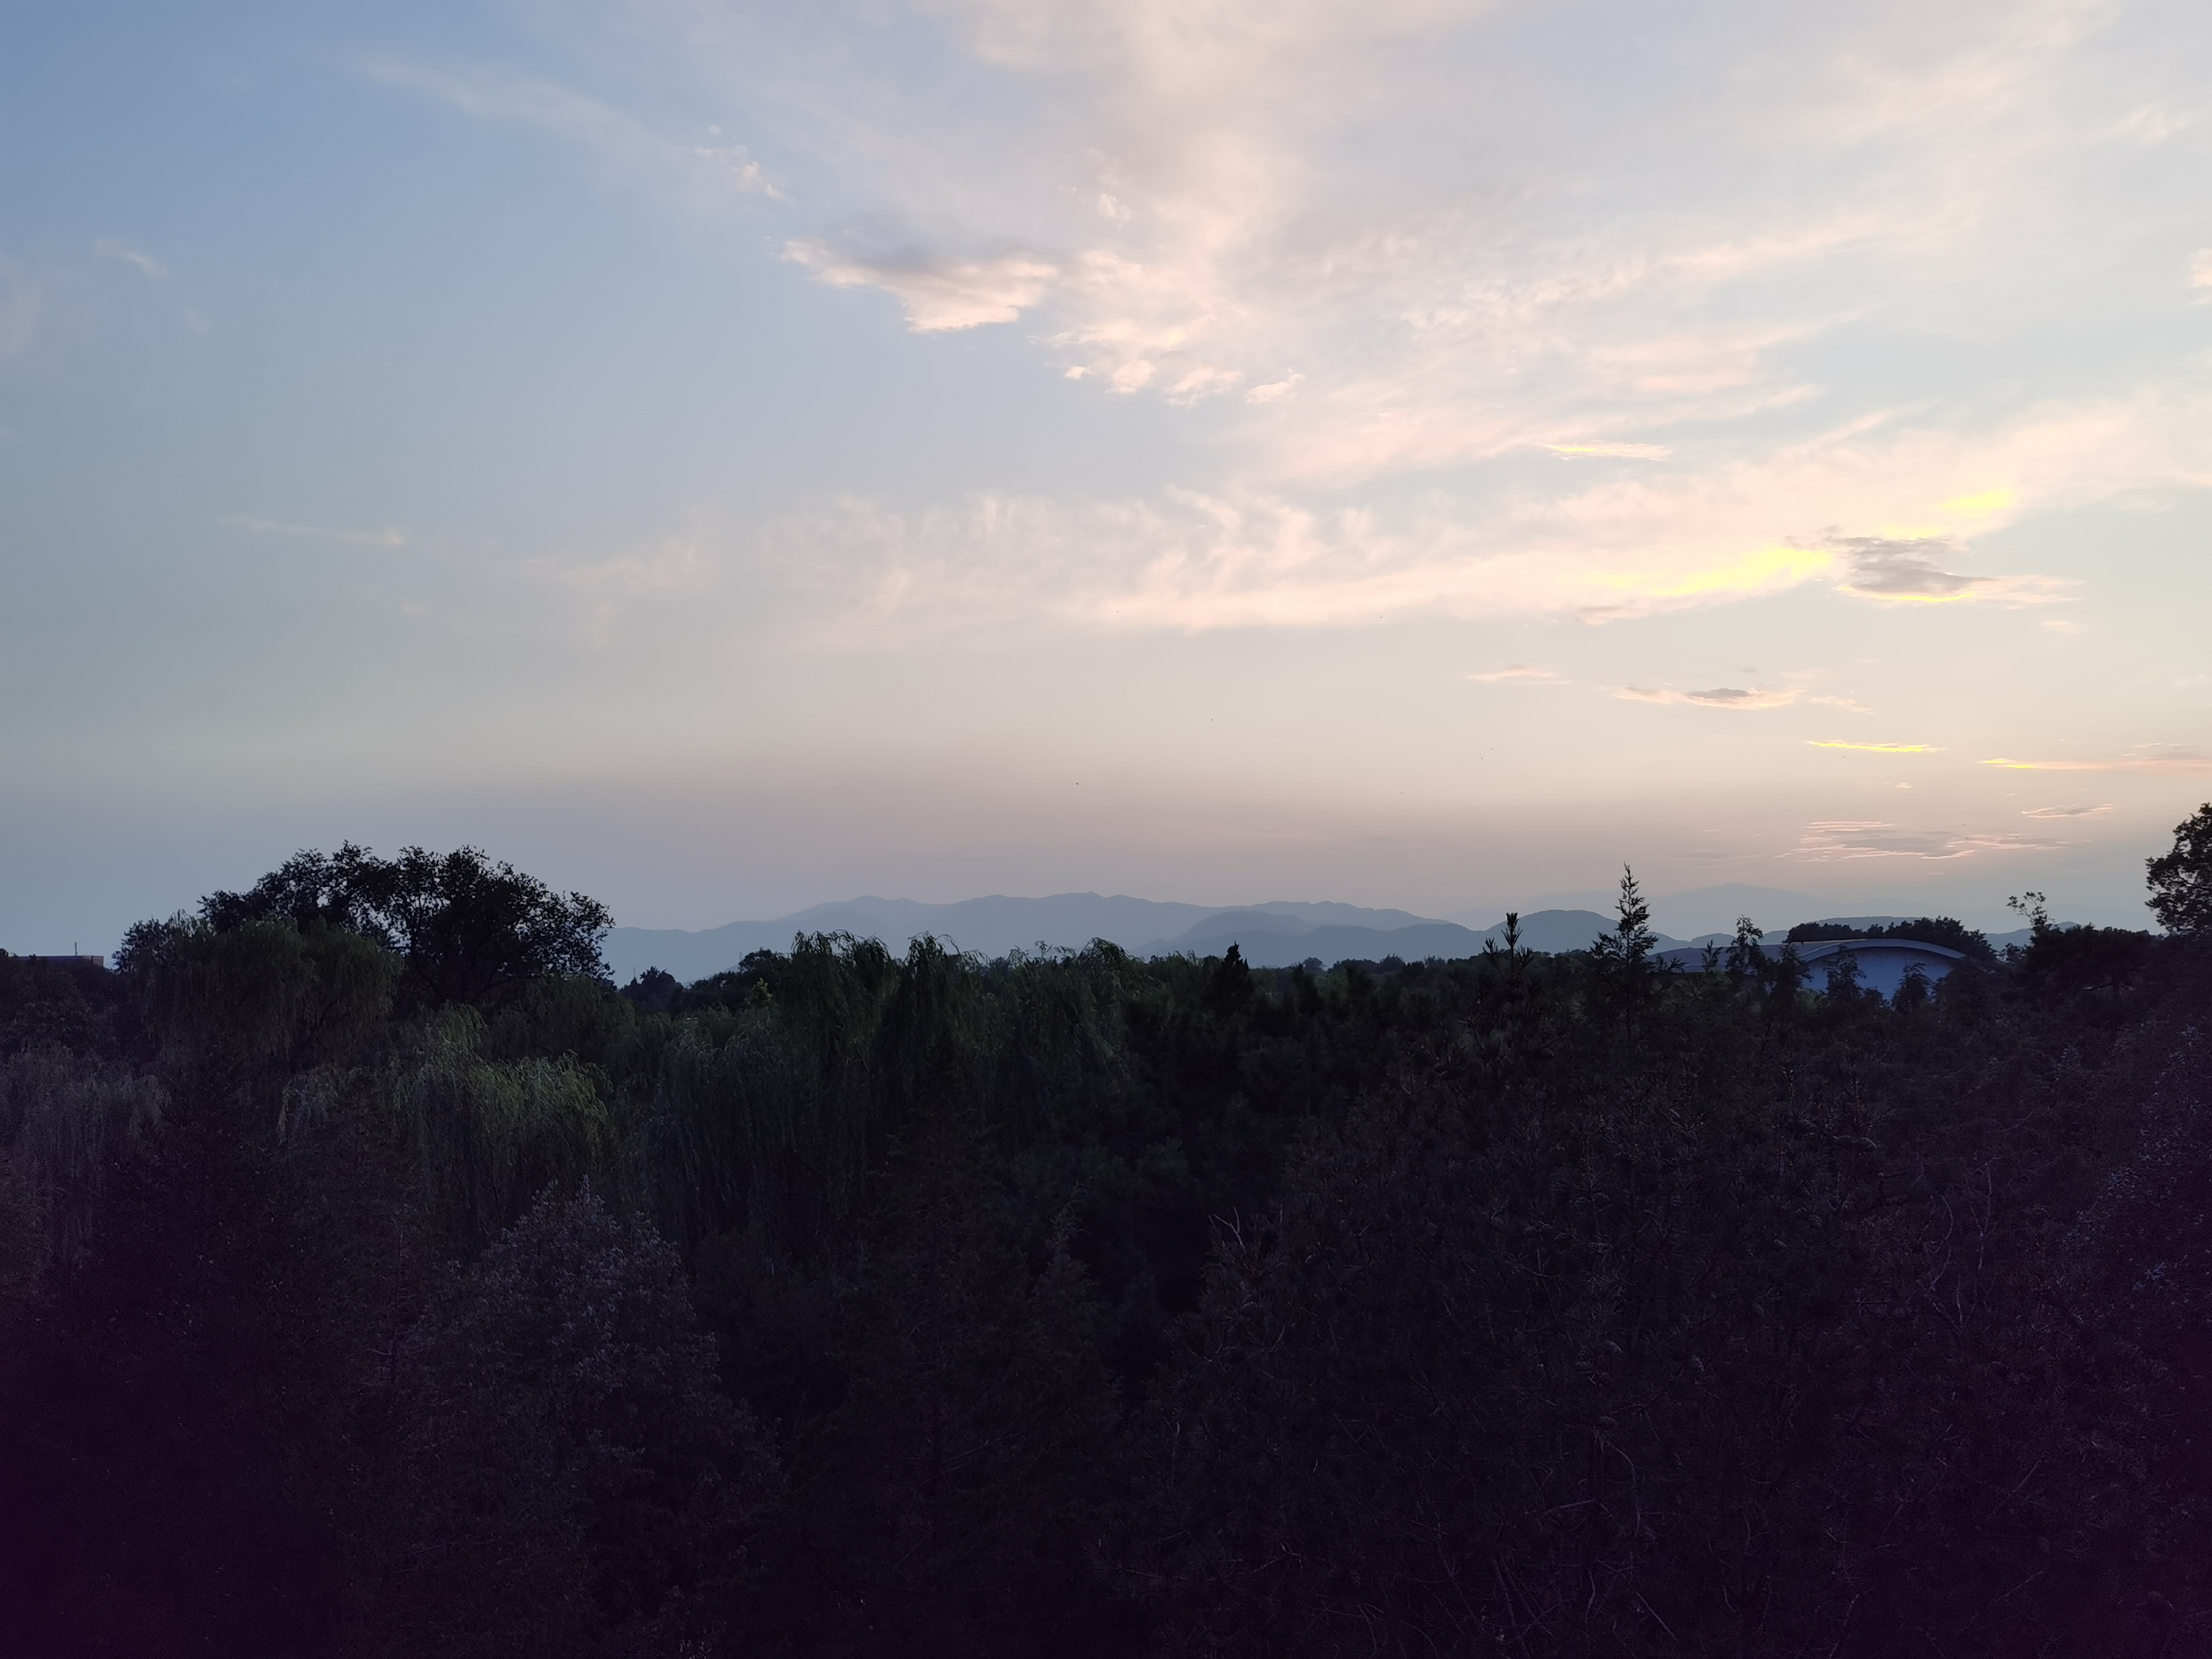
\includegraphics[width=\linewidth]{figures/零零阁暮望西山.jpg}
	从零零阁上远望西山。
\end{figure}

之前我与C君曾在阳光长跑时到过这个亭子。
当时跑得随性,只记得路过西湖附近,发现山上隐约有个亭子,便寻得路登了上去。穿过树丛,一座高大的亭子便豁然闯入眼帘。
我们正跑得气喘吁吁,然而登上二层后,阵阵凉风袭来,不胜清爽。
视野也陡然开阔。悠然东望,能从翠绿掩映中寻得六教深红的一角;极目向西,则甚至望得到远方巍巍西山:一时竟有种“一览众山小”的豪迈感,仿佛胸怀也随之变得更豁达了。
我们都对当时的场面印象深刻。于是C君提议,今日再登一次零零阁。

然而我们都已不记得这阁子的具体位置了,只大致记得应该是在荷塘旁靠近西湖的地方,于是我们便直奔荷塘而来。
荷塘北岸一马平川,自不可能有什么山巅的阁子。而湖心岛转过一遍,也没有发现符合当时印象的双层亭阁。
于是我们向荷塘南岸寻来。

荷塘这里靠近生活区,平时晚上就有许多人来这里散步、活动,因此相比园子里其他地方,有着浓浓的市井气息,仿佛城市里的公园一般。
然而晚上出来散步的人都聚集在荷塘北岸以及湖心岛的西北角,东面和南面的人烟便十分稀少,沿岸行走的话,仅间或能看到一两个默默垂钓的人。
我们沿荷塘东岸向南,至莲桥再向西。一过莲桥,就察觉这里人气已淡了许多。
太阳已经落山,又是阴天,浓云蔽月,再添上南岸茂密的树林,这时走在幽黑的林荫小径上,一阵凉风吹过,竟觉得有一些阴冷。
越向里走树木就越发茂密,光线也越来越暗,小径就仿佛没有出口的黑洞般,一直走不到尽头。这时我看到旁边有一条曲折延伸到山上密林中的小路。
微风吹过,我在这盛夏时节也不禁微微打了个寒颤,然后指着拐出去的小路说:“那亭子应该是在山顶上,我们一直沿着湖岸走要走到什么时候,不如往这里上去找一找。”C君亦以为然,于是我们便向山上走去。

\begin{figure}[!h]
	\centering
	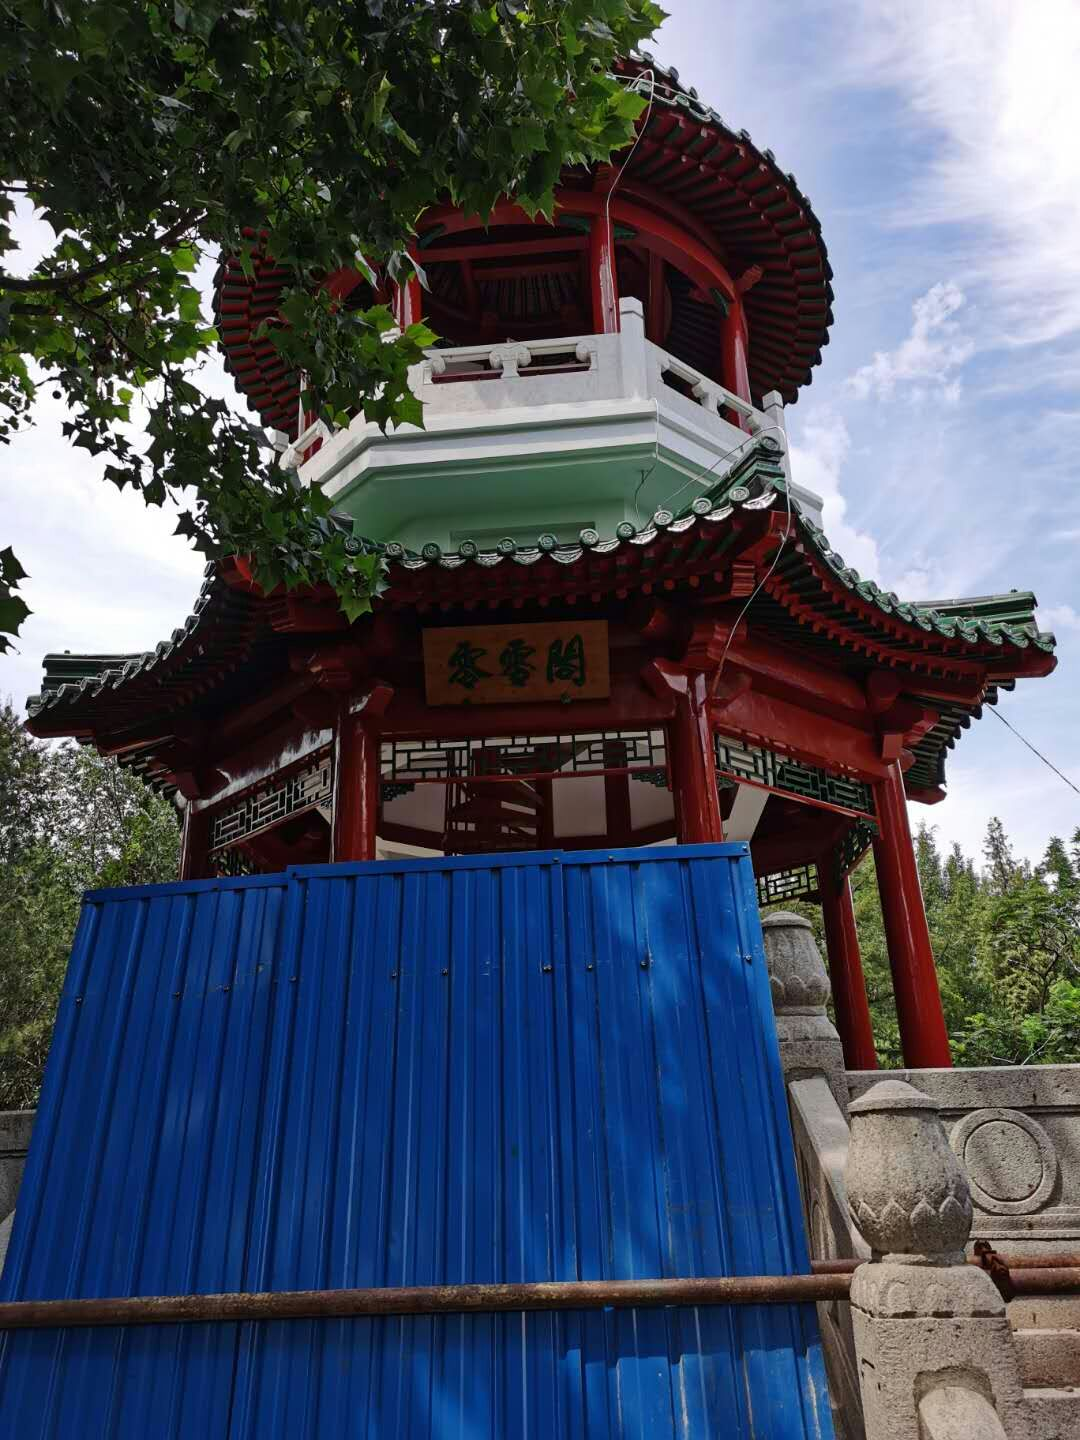
\includegraphics[width=\linewidth]{figures/零零阁.jpg}
	零零阁
\end{figure}

上山的小路坑坑洼洼的,许多铺路的石块都缺失了,表面还散布着细碎的石子,给人久未维护的感觉。
靠近山顶,树林稍稍稀疏了些,能够看到天上的阴云,也能看到前方朦胧的建筑,零零阁就在眼前了。
我们喜出望外,急忙沿着山路跑到了尽头,来到了心心念念的零零阁前,却惊讶地发现山路被围挡折断,亭子已整个被包围在其中,显然是正在翻修,无法再上去一瞰清华。大失所望之际,我们也只好再折返下山去。
这时一阵风穿过树林,发出尖锐的啸声,我们俩不禁又打了个哆嗦,不觉间已加快了下山的脚步。

就要走出湖边的小道时,迎面走来了一个满身酒气的人。
小径狭窄,几乎容不下他踉跄的步伐,我们只好赶紧闪到路边草坪上,让他先行过去。
兴许是刚刚赴完局,打算饭后找个清静少人的地方散散步,消消食,醒醒酒,随后便回家去,所以他也不顾夜色已深,便晃悠悠地走进了林荫小道,向荷塘南边走去。
素不相识,他的事,自然与我们无关,因而我们出来后,找到自己的自行车,便匆匆离去了。
当晚无事。

然而三天后的中午,C君突然急匆匆地找到我,递给我一份当日的报纸。
我低头一看,一下子就被报纸上的一条消息吓到了:
“昨日北京市某大学校内小山上某施工地点附近发现一具无头男尸,死状凄惨,全身血液流失殆尽。
法医初步鉴定死亡时间为两天前凌晨时段。
目前案件正在进一步调查中。”
报上黑白的配图虽然有些模糊,但我还是立刻就认出,那正是零零阁所在的那座小山……

\vfill

\paragraph{记事}
6月23日傍晚,笔者约C君出来共游校园,途中C君提到想再上一次零零阁,于是二人往西湖与荷塘这边寻来。
寻觅良久,终于在荷塘南边的小山上找到了亭子,却发现亭子已被围起来翻修了,失望而归。
